Durante l'analisi del contenuto del filesystem effettuata con Autopsy, è stato evidenziato come sospetto il file \textbf{Important Document.zip}, presente nella directory\\
\texttt{C:/Users/Laura/Desktop}. Il motivo della segnalazione del file è dovuto ad un'alta entropia dei suoi contenuti, suggerendo che il file fosse criptato.\\
Eseguendo infatti il comando per calcolare l'entropia del contenuto di un file:
\begin{center}
    \texttt{ent Important Document.zip}
\end{center}
si ottiene il valore \textbf{7.999983} bits per byte, indicando che i bit sono distribuiti uniformemente nel contenuto, quasi vicino al massimo teorico di 8.\vspace{14pt}\\
Supponendo dunque che il file fosse criptato abbiamo provato ad identificare il tipo di cifratura utilizzando \textbf{hashcat}, eseguendo il comando:
\begin{center}
    \texttt{hashcat Important Document.zip}
\end{center}
L'assenza di header o di una lunghezza specifica del file non suggeriscono una tipologia specifica di cifratura, indicando dunque che si tratta di una full-text-encryption effettuata con algoritmi come \textbf{VeraCrypt} o \textbf{TrueCrypt}.\\
Data la numerosità di algoritmi di cifratura di questo tipo abbiamo deciso di non procedere con la decifrazione del contenuto in bruteforce, ma piuttosto analizzare altre strade.\vspace{14pt}\\
Il sistema operativo Windows permette agli utenti di cifrare un file con una chiave che è generata a partire dalle informazioni di login dell'utente. La cifratura del file appare trasparente all'utente in quanto dopo aver effettuato il login il file viene "\textit{sbloccato}". In eventuali acquisizioni forensi dunque il file verrà mostrato nella sua natura criptata.\vspace{14pt}\\
Per poter accedere al file è dunque necessario effettuare il login come Laura. Abbiamo deciso di effettuare il boot del disco.\vspace{14pt}\\
A partire da un'immagine \textbf{E01} non è immediato il processo di boot, abbiamo quindi effettuato diversi tentativi:
\subsubsection{FTKImager + VirtualBox}
Abbiamo utilizzato FTKImager per espandere l'immagine nelle sue totali dimensioni di `500GB` in modo da poter montare fisicamente il disco sulla nostra macchina locale.\\
In seguito abbiamo utilizzato il tool \textbf{VBoxManage.exe} per poter generare un file \textbf{.vmdk} che facesse da link per la macchina virtuale con il disco montato.\\
La creazione del file .vmdk non è però andata a buon fine.
\subsubsection{Arsenal Image Mounter + VMWare Workstation}
Il secondo tentativo è stato quello di utilizzare \textbf{Arsenal Image Mounter} per creare il disco su cui eseguire il boot della VM. La peculiarità di Arsenal è che riesce a montare il disco partendo da un E01, con scrittura abilitata, mantenendolo offline.
\begin{center}
    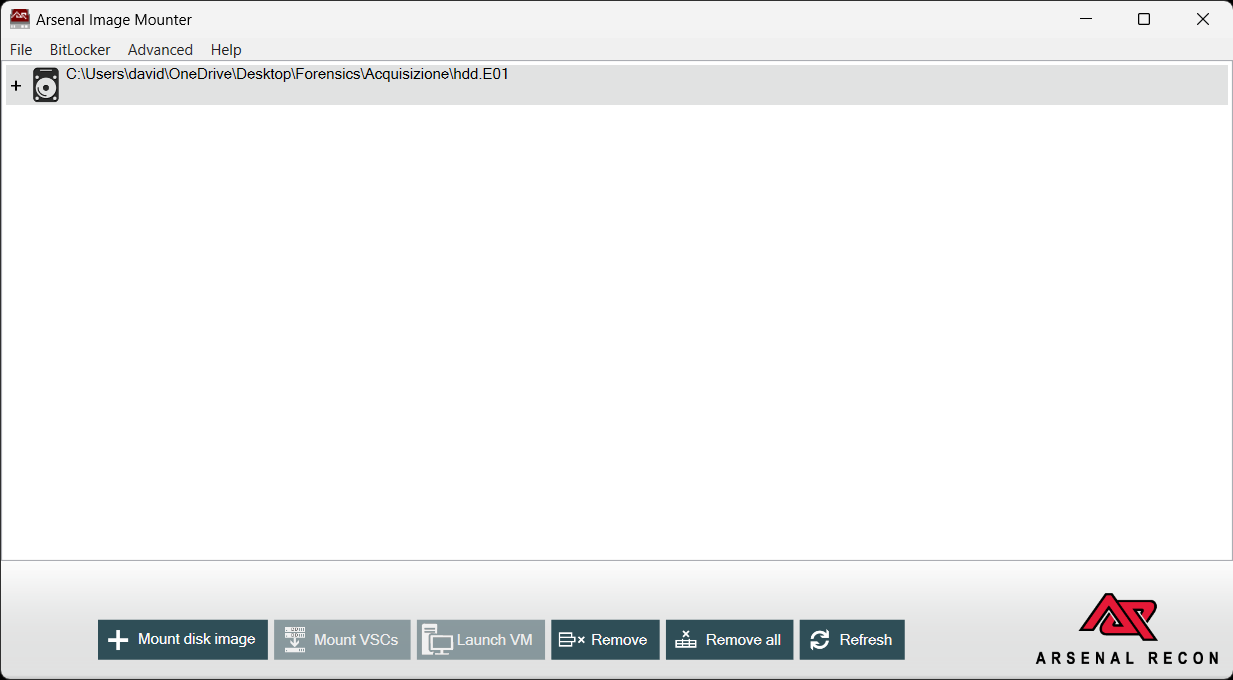
\includegraphics[width=0.8\textwidth]{img/arsenal-imager.png}
\end{center}
Per evitare che il file E01 venisse modificato abbiamo specificato una posizione di write cache dove i cambiamenti effettuati sulla VM vengono salvati.\\
Arsenal ha dunque montato il disco offline \textbf{PhysicalDrive1} da cui siamo riusciti a creare la virtual machine utilizzando \textbf{VMWare Workstation}.\vspace{14pt}\\
Durante la creazione della VM abbiamo dovuto configurare diversi parametri. In questa fase sono stati effettuati diversi tentativi (non funzionanti). Dopo svariate ore e prove siamo arrivati ad una combinazione di parametri funzionanti, confermati anche da valori trovati su Autopsy:
\begin{itemize}
    \item \textbf{Distribuzione del Sistema Operativo}: Windows 7 Professional
    \item \textbf{Architettura}: x86 32Bit
    \item \textbf{Interfaccia Disco}: SATA
    \item \textbf{Memoria RAM}: 1Gb
    \item \textbf{Numero Processori}: 1 
\end{itemize}
Con questi parametri, la VM ha effettuato un boot funzionante senza schermate \textbf{BSOD} che precedentemente hanno invalidato i diversi tentativi effettuati.
\begin{center}
    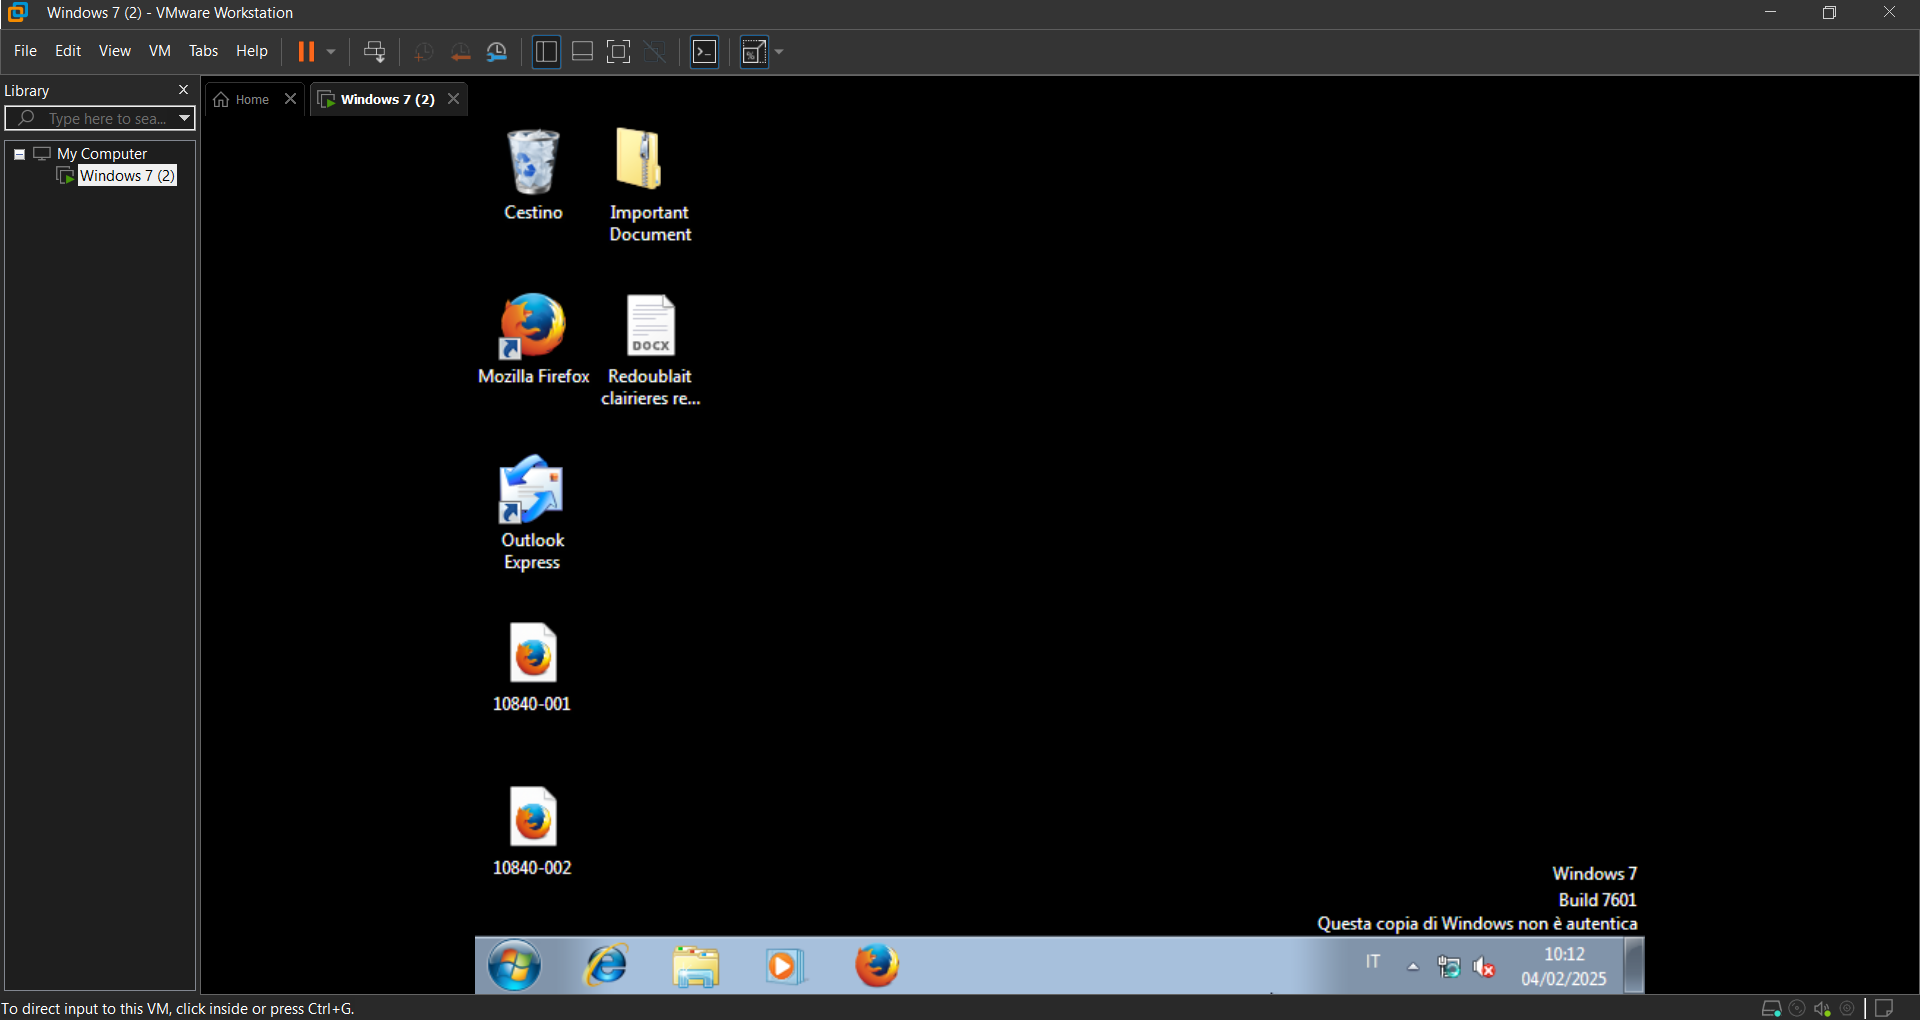
\includegraphics[width=1\textwidth]{img/live.png}
\end{center}
E' possibile osservare l'utente Laura.
\begin{center}
    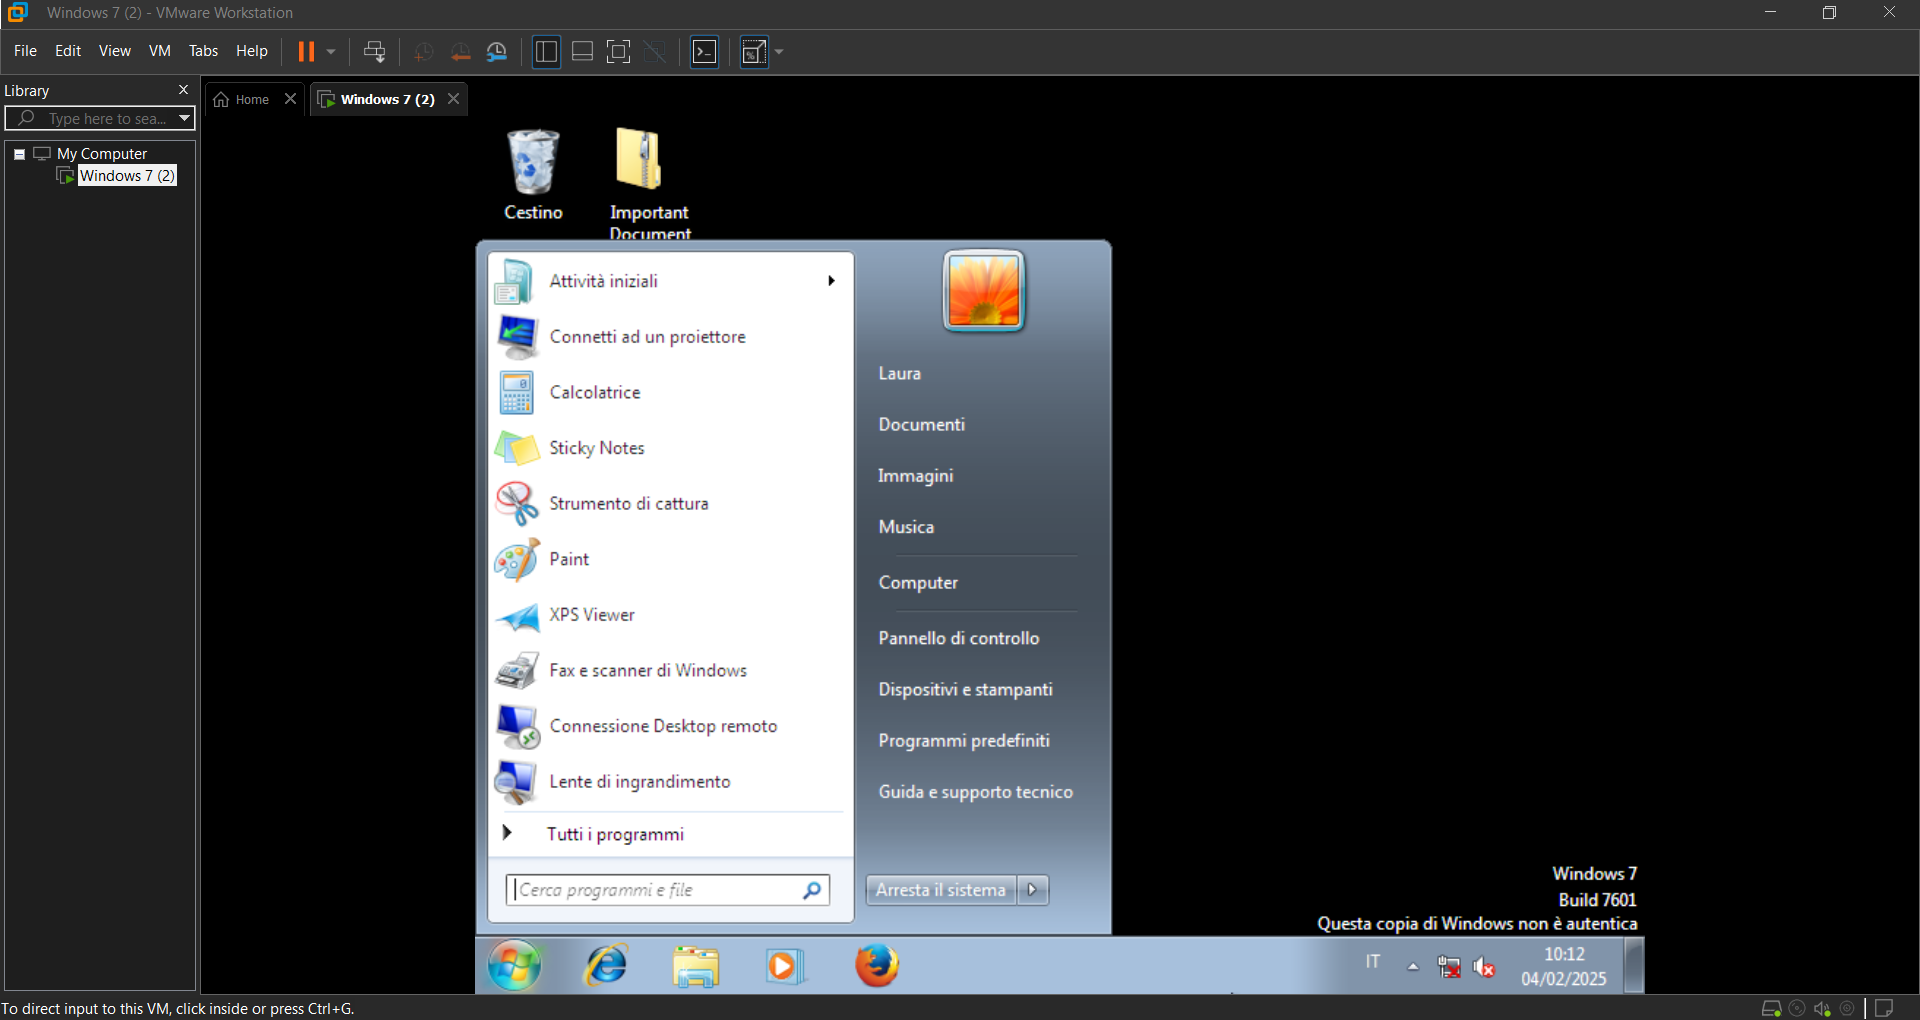
\includegraphics[width=1\textwidth]{img/live-laura.png}\vspace{100pt}\\
\end{center}
Provando quindi ad aprire il file Important Document.zip dall'utente Laura notiamo il messaggio di errore restituito.
\begin{center}
    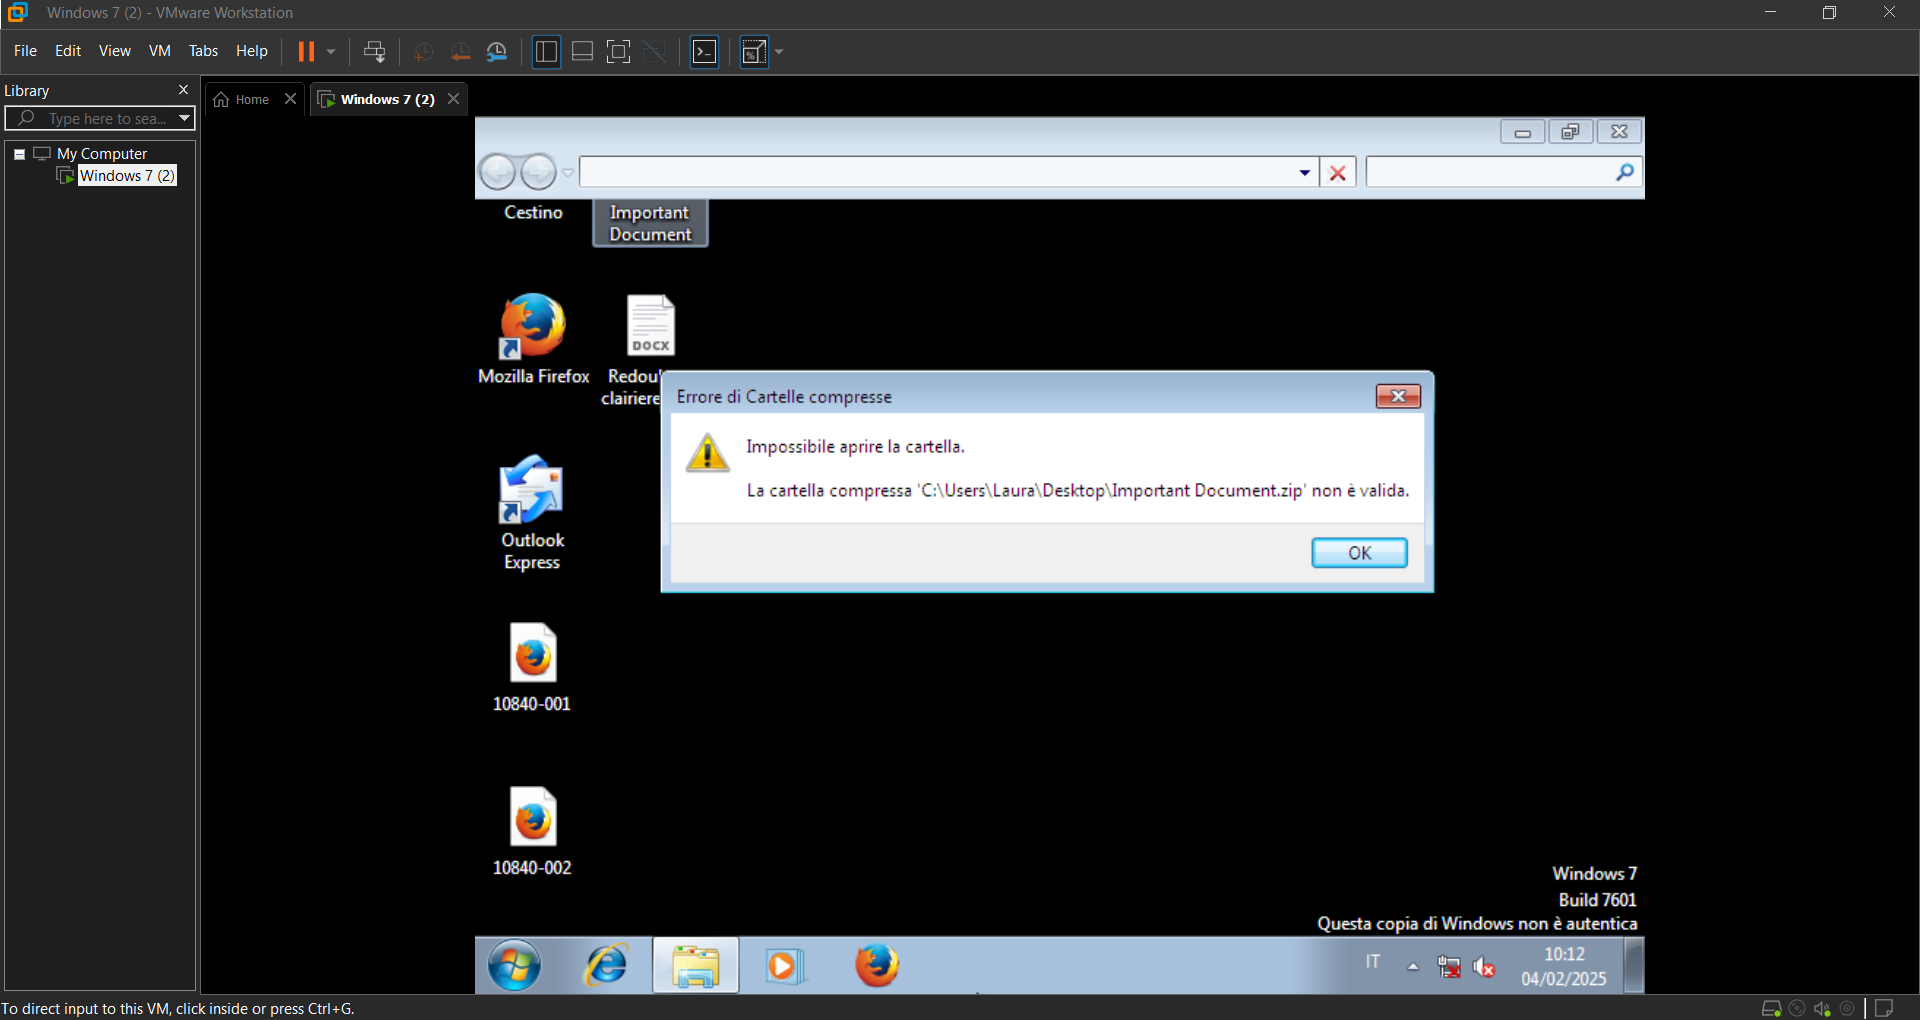
\includegraphics[width=1\textwidth]{img/important-fail.png}
\end{center}